% mnras_template.tex 
%
% LaTeX template for creating an MNRAS paper
%
% v3.0 released 14 May 2015
% (version numbers match those of mnras.cls)
%
% Copyright (C) Royal Astronomical Society 2015
% Authors:
% Keith T. Smith (Royal Astronomical Society)

% Change log
%
% v3.0 May 2015
%    Renamed to match the new package name
%    Version number matches mnras.cls
%    A few minor tweaks to wording
% v1.0 September 2013
%    Beta testing only - never publicly released
%    First version: a simple (ish) template for creating an MNRAS paper

%%%%%%%%%%%%%%%%%%%%%%%%%%%%%%%%%%%%%%%%%%%%%%%%%%
% Basic setup. Most papers should leave these options alone.
\documentclass[fleqn,usenatbib]{mnras}

% MNRAS is set in Times font. If you don't have this installed (most LaTeX
% installations will be fine) or prefer the old Computer Modern fonts, comment
% out the following line
\usepackage{newtxtext,newtxmath}
% Depending on your LaTeX fonts installation, you might get better results with one of these:
%\usepackage{mathptmx}
%\usepackage{txfonts}

% Use vector fonts, so it zooms properly in on-screen viewing software
% Don't change these lines unless you know what you are doing
\usepackage[T1]{fontenc}
\usepackage{ae,aecompl}


%%%%% AUTHORS - PLACE YOUR OWN PACKAGES HERE %%%%%

% Only include extra packages if you really need them. Common packages are:
\usepackage{graphicx}	% Including figure files
\usepackage{amsmath}	% Advanced maths commands
\usepackage{amssymb}	% Extra maths symbols

%%%%%%%%%%%%%%%%%%%%%%%%%%%%%%%%%%%%%%%%%%%%%%%%%%

%%%%% AUTHORS - PLACE YOUR OWN COMMANDS HERE %%%%%

% Please keep new commands to a minimum, and use \newcommand not \def to avoid
% overwriting existing commands. Example:
%\newcommand{\pcm}{\,cm$^{-2}$}	% per cm-squared

%%%%%%%%%%%%%%%%%%%%%%%%%%%%%%%%%%%%%%%%%%%%%%%%%%

%%%%%%%%%%%%%%%%%%% TITLE PAGE %%%%%%%%%%%%%%%%%%%

% Title of the paper, and the short title which is used in the headers.
% Keep the title short and informative.
\title[Hercules-Aquila and Virgo Clouds with Gaia DR2]{Hercules-Aquila
  and Virgo Clouds with Gaia DR2. Evidence for a common origin}

% The list of authors, and the short list which is used in the headers.
% If you need two or more lines of authors, add an extra line using \newauthor

\author[Iulia T. Simion et al]{Iulia T. Simion$^{1}\thanks{E-mail:isimion@shao.ac.cn}$, Vasily Belokurov$^{2,3}$ and  Sergey E. Koposov$^{2,4}$\\
  $^{1}$Key Laboratory for Research in Galaxies and Cosmology, Shanghai Astronomical Observatory, 80 Nandan Road, Shanghai 200030, China\\
  $^{2}$Institute of Astronomy, Madingley Rd, Cambridge, CB3 0HA\\
  $^{3}$Center for Computational Astrophysics, Flatiron Institute, 162 5th Avenue, New York, NY 10010, USA\\
  $^4$Department of Physics, McWilliams Center for Cosmology, Carnegie Mellon University, 5000 Forbes Avenue, Pittsburgh, PA 15213, USA
}

% These dates will be filled out by the publisher
\date{Accepted XXX. Received YYY; in original form ZZZ}

% Enter the current year, for the copyright statements etc.
\pubyear{2018}

% Don't change these lines
\begin{document}
\label{firstpage}
\pagerange{\pageref{firstpage}--\pageref{lastpage}}
\maketitle

% Abstract of the paper
\begin{abstract}
200 words for Letters.
No references should appear in the abstract.
\end{abstract}

% Select between one and six entries from the list of approved keywords.
% Don't make up new ones.
\begin{keywords}
keyword1 -- keyword2 -- keyword3
\end{keywords}

%%%%%%%%%%%%%%%%%%%%%%%%%%%%%%%%%%%%%%%%%%%%%%%%%%

%%%%%%%%%%%%%%%%% BODY OF PAPER %%%%%%%%%%%%%%%%%%

\section{Introduction}

How do you hide the evidence for a massive impact event that caused
the extinction of most of the dinosaurs as well as 75\% of all species
on Earth? You bury it deep under the sea, covered with a layer of
sediment taller than the Empire State Building
\citep[][]{Hildebrand1991}. Without the discovery of the giant
Chicxulub crater, the meteorite impact hypothesis would remain a neat
theory supported by striking but indirect evidence. A hypothesis of an
ancient dramatic collision between the Milky Way and an unidentified
massive dwarf galaxy was put forward by \citet{Deason2013} to explain
a particular feature in the overall stellar halo density profile
\citep[][]{Wa09,De11}. Most recently, through a study of a portion of
the nearby stellar halo, \citet{Belokurov2018} demonstrated that the
great impactor must have collided with the young Milky Way on a nearly
radial orbit, thus swamping the inner stellar halo with metal-rich
material with orbital anisotropy \citep[see][]{Binney2008} close to
unity. Merger events like this tend to leave behind a battery of
debris clouds and shells \citep[see][]{Amorisco2015,Hendel2015}, which
- akin to the peak rings of impact craters \citep[see
  e.g.][]{Morgan2016} - if discovered could help to reconstruct the
collision as well as pin down the properties of the progenitor
\citep[e.g][]{Sanderson2013,Johnston2016}.

Before the Data Release 2 \citep[][]{Brown2018} of the ESA's Gaia
mission \citep[][]{Prusti2016}, five large and diffuse cloud-like
structures had been discovered in the Galaxy's halo. These include:
the Virgo Over-Density
\citep[VOD,][]{Vivas2001,Newberg2002,Duffau2006,Juric2008,Bonaca2012},
the Hercules-Aquila Cloud \citep[HAC,][]{Be07,Simion2014}, the
Trinagulum-Andromeda structure
\citep[Tri-And,][]{Rocha2004,Majewski2004,Deason2014}, the Pisces
Over-density \citep[][]{Sesar2007,Wa09,Nie2015} and the
Eridanus-Phoenix over-density \citep[Eri-Pho,][]{Li2016}. According to
the most recent investigations, Tri-And likely comprises of Galactic
disc stars kicked out of the plane in a recent interaction with a
dwarf galaxy, probably the Sagittarius dSph
\citep[e.g.][]{Pr15,Bergemann2018,Hayes2018}. Of the remaining four,
the Pisces overdensity clearly stands out as it reaches much larger
Galacto-centric distances. On the other hand, the VOD, HAC and Eri-Pho
structures occupy a very similar range of distances, between 10 and 20
kpc from the Galactic center. This lead \citet{Li2016} to suggest that
these three Clouds could all be part of one merger event, a galaxy
accreted onto the Milky Way on a polar orbit \citep[see
  also][]{Juric2008}.

As demonstrated by the recent re-interpretation of the Monoceros Ring
(and the associated sub-structures) and the Tri-And, deciphering the
nature of halo over-densities is often impossible without either
high-resolution spectroscopy \citep[e.g.][]{Bergemann2018} or accurate
astrometry \citep[e.g.][]{deBoer2018,Deason2018}. In this Letter, we
look for clues to the formation of the Hercules-Aquila and Virgo
Clouds using proper motions provided as part of the Gaia DR2. At our
disposal are highly pure samples of members of each Cloud, namely the
RR Lyrae stars that i) are co-spatial with HAC and VOD in 3-D and ii)
that have their line-of-sight velocities measured. By complementing
the publicly available 4-D data with the GDR2 proper motions, we build
a large tracer set with complete 6-D phase space information and study
the make-up of each structure using the orbital properties of the
constituent stars.

\section{Data and analysis}
%
\begin{figure}
	% To include a figure from a file named example.*
	% Allowable file formats are eps or ps if compiling using latex
	% or pdf, png, jpg if compiling using pdflatex
	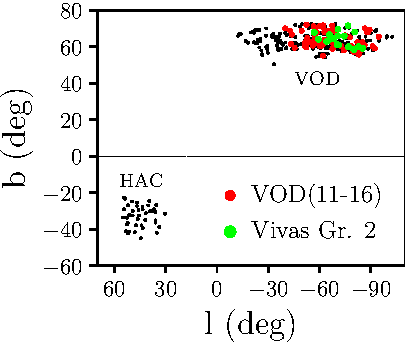
\includegraphics[scale=0.515]{lb.pdf}
	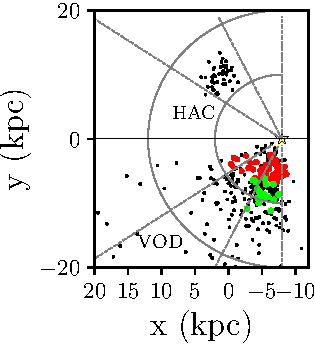
\includegraphics[scale=0.515]{xy.pdf}
	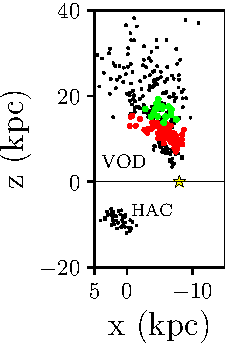
\includegraphics[scale=0.515]{xz.pdf}
	\vspace{-0.4cm}
    \caption{Spatial distribution of the RR Lyrae used in this work with full 6-D phase space measurements, in Galactic coordinates (left panel) and in the $x-y$ (middle) and $y-z$ (right) planes.  The HAC field contains 44 RR Lyrae which likely belong to the Cloud with measured line-of-sight  velocities (Simion et al. 2018) and  Gaia DR2 proper motions. The VOD field contains 411 RRL which belong to several halo associations, including the Sagittarius stream and the VOD, with line-of-sight velocities provided by Vivas et al. 2016 and proper motions from Gaia DR2. In particular we mark group 2, a `high significance' kinematical group, which contains 18 stars (green circles). The semi-circles are centred on the Sun's position and have radius of 10 and 20 kpc. The Sun (yellow star) is located at (x$_{\odot}$, y$_{\odot}$, z$_{\odot})= $ (0,-8,0) kpc and the Galactic centre at (0,0,0) - black circle.  }
    \label{fig:lb}
\end{figure}
%

\subsection{4-D RR Lyrae data}

The Hercules-Aquila and Virgo Clouds are diffuse stellar
over-densities in the inner stellar halo, located on the opposite
sides of the Galaxy (see Figure~\ref{fig:lb}). At high latitudes,
these are detected as peaks in RR Lyrae number counts - curiously - at
similar heliocentric distances, i.e. $\sim$17 kpc (HAC:
\citealt{Wa09,Simion2014}) and $\sim$19 kpc (VOD: \citealt{Vivas2006,
  Duffau2014, Vivas2016}). Note that other tracers (e.g. BHBs, MSTO
and K and M giants) have also been used to pin down the morphology of
the Clouds \citep[see
  e.g.][]{Be07,Juric2008,Sharma2010,Bonaca2012,Conroy2018}. The RR
Lyrae, however offer the clearest view of these halo sub-structures
thanks to the associated accurate distances and minuscule Galactic
foreground contamination. Therefore, in this work, we have focused on
the two recently published samples of RR Lyrae towards the Clouds,
where each star has a well-measured line-of-sight velocity.

\begin{itemize}
\item \citet{Simion2018} provide a table of 46 RRL with radial
  velocity measurements (45 observed with MDM and 1 from SDSS) with
  heliocentric distances between 15 and 18 kpc;
\item \cite{Vivas2016} compiled a catalog of 412 RRL in the region of
  the sky covered by the VOD with distances between 4 and 75 kpc from
  the Sun with radial velocity measurements of stars from La
  Silla-QUEST, QUEST, CRTS and LINEAR.
\end{itemize}

%
\subsection{From 4-D to 6-D. Velocity distributions}

By cross-matching to the GDR2 data with an aperture of 2$''$, we have
found Gaia counterparts to 44 HAC stars and 411 VOD. From the VOD
sample, we remove 112 stars likely belonging to the Sgr stream as
identified by \citep[][, their group 1]{Vivas2016}. The spatial
distribution of the remaining stars (44 from \citealt{Simion2018} and
299 from \citealt{Vivas2016}) with full 6-D phase space measurements
is given in Figure~\ref{fig:lb}, in Galactic coordinates in the left
panel and in the x-y (x-z) Galactic plane in the middle (right)
panel. We adopt a left-handed Galactic Cartesian coordinates with the
Sun located at (x$_{\odot}$,y$_{\odot}$, z$_{\odot}$) = (-8,0,0) kpc,
the x-axis positive in the direction of the Galactic center, y-axis
oriented along the Galactic rotation and the z-axis directed towards
the north Galactic pole. While \citealt{Vivas2016} identify 6
significant kinematical groups in the VOD region (their Table 5), only
groups 1 (Sagittarius stream) and 2 (likely members of the VOD, with
$\mathrm{<v_{GSR}>}= 135$ km/s) contain more than 10 stars. We mark
group 2 with green circles in Figure~\ref{fig:lb}. We also mark with
red circles the location of a group of stars selected to have
galactocentric distances similar to the HAC sample, i.e.
$11\mathrm{<r_{GC}}/$kpc$<16$ to facilitate a fair comparison of their
velocities and orbits.

%
\begin{figure}
	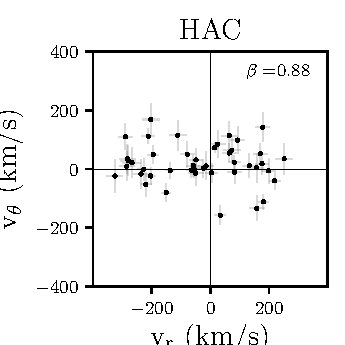
\includegraphics[scale=0.53]{HAC_velocities_vphi.pdf}
    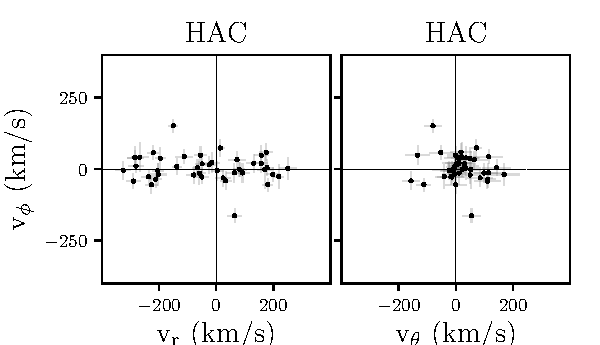
\includegraphics[scale=0.53]{HAC_velocities_vtheta.pdf} 
  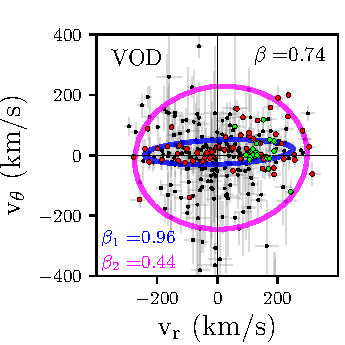
\includegraphics[scale=0.53]{VOD_velocities_vphi.pdf}
    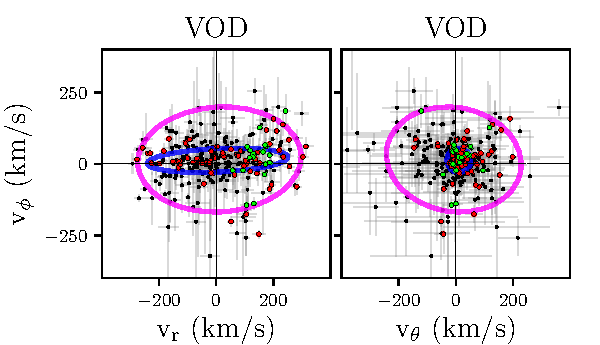
\includegraphics[scale=0.53]{VOD_velocities_vtheta.pdf}  
\vspace{-0.4cm}
    \caption{RRL velocity distribution in spherical polar coordinates
      ($v_{r}$, $v_{\theta}$, $v_{\phi}$ are the radial, azimuthal and
      polar components respectively) in the HAC field (top row) and
      the VOD field (middle and bottom rows). The error on the
      velocity components of each star $i $, [$\sigma^{i}_{v_{r}}$,
        $\sigma^{i}_{v_{\theta}}$, $\sigma^{i}_{v_{\phi}}$], has been
      propagated by randomly drawing 1000 stars from a multivariate
      Gaussian distribution with mean the measurement (ra$^{i}$,
      dec$^{i}$, d$^{i}$, pmra$^{i}$, pmdec$^{i}$, $v^{i}_{h}$) and
      full covariance matrix (takes into account the covariances
      between ra,dec and proper motions). The orbital anisotropy, is
      highly radial in the HAC field ($\beta = 0.91 \pm 0.03$) where
      the stars are most likely members of the Cloud and mildly radial
      in the VOD field ($\beta = 0.74 \pm 0.04$) in which stars span a
      much wider range of distances (see Fig. \ref{fig:lb}). }
    \label{fig:vel}
\end{figure}
%

%
\begin{figure}
	\hspace{-0.3cm}
	        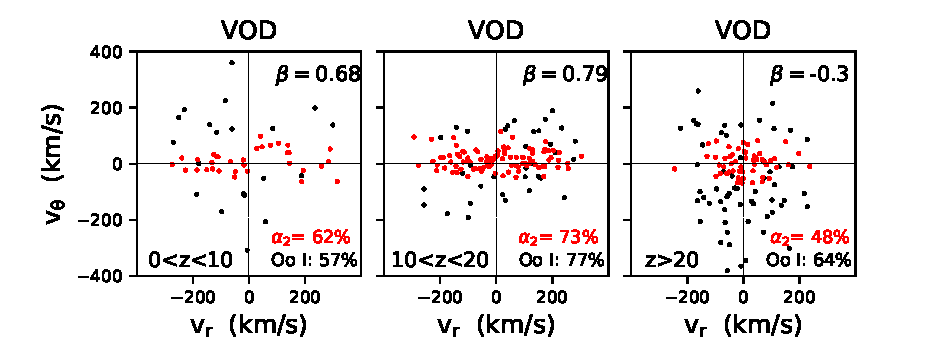
\includegraphics[scale=0.56]{VOD_velocities_vphi_zcuts.pdf}
\vspace{-0.4cm}
   \caption{Radial versus azimuthal velocity in the VOD field, in
     three distance ranges above the Galactic plane. The fraction of
     RR Lyrae of Oosterhoff type I is reported in each panel. }
    \label{fig:VOD_vel}
\end{figure}
%

Figure~\ref{fig:vel} shows the spherical polar components of the
velocities (radial $v_{r}$, azimuthal $v_{\theta}$ and polar
$v_{\phi}$) of stars in the HAC (top row) and VOD (bottom row)
fields. Group 2 stars (green) can be seen clustering at $v_{r} = 135$
km/s (by design), while the stars at intermediate $\mathrm{r_{GC}}$
(red) seem to have a velocity distribution very similar to those in
the HAC, shown in the top row. To estimate the uncertainty in each
velocity component we propagate the measured proper motion and
line-of-sight velocity errors using Monte-Carlo re-sampling, where we
take into account the covariances between the measurements of the
Right Ascension and Declination components of proper motion as
provided in GDR2. We use the standard deviations of the resulting
\{$v_{r}$, $v_{\theta}$, $v_{\phi}$\} distributions as the upper limits
of the velocity uncertainties; these are shown in Fig.~\ref{fig:vel}.

%add comments on the size of the errorbars; standard deviation
%works well I think here, distributions quite gaussian. didn't work
%well for the anisotropy later on, there I used the percentiles

As evident from the Figure, the velocity distributions are highly
anisotropic, with the dispersion in the radial component dominating
the tangential ones, especially in the HAC data. To describe the shape
of the velocity distributions, we model each stellar sample as a
single-component multi-variate Gaussian using the Extreme
Deconvolution module implemented in $\mathrm{astroML}$
\citep{astroML}. The resulting parameters and the associated
uncertainties of the velocity ellipsoids are taken to be the median
and the standard deviation values of 500 bootstrap re-sampling trials.
The velocity ellipsoid shape can be summarized using the anisotropy
parameter $\beta=1-(\sigma^2_{\theta}+\sigma^2_{\phi})/2\sigma^2_r$
\citep[see][]{Binney2008}. We find the HAC stars have radially biased
orbits with $\beta = 0.91 \pm 0.03$ while for the whole of the VOD
sample, $\beta = 0.74 \pm 0.04$). Note, however, that the two samples
span very different ranges in Galactic $l,b$ and distances. According
to \citet{Belokurov2018}, the inner stellar halo can be viewed as a
mixture of two debris components with distinct
properties. Accordingly, we fit a model with two multivariate
Gaussians to the VOD velocity data using Extreme Deconvolution
\citep[see][]{ED}. The VOD sample appears to be composed of roughly
two thirds of stars with $\beta_{1}= 0.96^{+0.02}_{-0.44}$ (marked in
magenta in Fig. \ref{fig:vel}) and a third with
$\beta_{2}=0.44^{+0.45}_{-0.20}$ (blue) in good agreement with the
results for the local halo presented in \citet{Belokurov2018}.

Using virial theorem, \citet{actionhalo} concluded that the radially
anisotropic component of the stellar halo is also significantly
flattened vertically. To test this hypothesis, we split the VOD sample
into 3 groups according to their distance from the Galactic plane and
show the behaviour of the azimuthal $v_{\theta}$ and radial $v_{r}$
velocity distributions in Figure~\ref{fig:VOD_vel}. Additionally, for
each z slice we have calculated the fraction of Oosterhoff type I (Oo
I) RR Lyrae, using equations 1 and 2 in \citet{Be2018} to explore the
changes in the RRL mixture. In the 10$<$z/kpc$<$20 range, where the
velocity anisotropy is the highest ($\beta = 0.84 \pm 0.03$)
approaching the value in the HAC field, the Oo I type dominates
(77\%). In the same slice, 73\% of the stars belong to the more
squashed (or `sausage' looking) velocity ellipsoid. The same behaviour
but less accentuated can be noticed in the 0$<$z/kpc$<$10 slice where
the anisotropy $\beta = 0.7 \pm 0.1$ is lower but the fraction of Oo I
stars is somewhat lower at 57\%. Further from the plane, at z$>$20
kpc, the velocity ellipsoid changes dramatically to almost isotropic
with $\beta = -0.1 \pm 0.2$. Please note that in this particular z
bin, the $\beta$ value may still be affected by the presence of the
Sagittarius stream. Group 2 and the stars sharing the same
galactocentric distance range with the HAC, are all located at $z<20$
kpc. Interestingly, the HAC counterparts in the VOD (red points) are
all clearly part of the anisotropic component.

% 
\subsection{Orbital properties of the HAC and VOD}
%
\begin{figure}
	% To include a figure from a file named example.*
	% Allowable file formats are eps or ps if compiling using latex
	% or pdf, png, jpg if compiling using pdflatex
	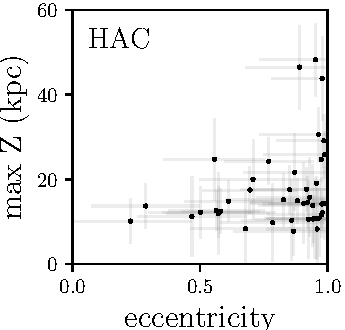
\includegraphics[scale=0.473]{HAC_orbits_ecc_z.pdf}
    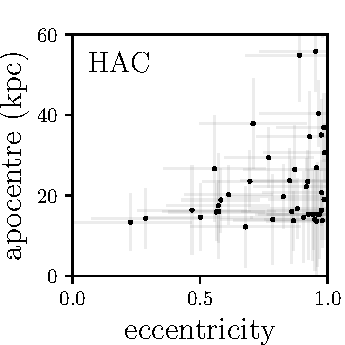
\includegraphics[scale=0.473]{HAC_orbits_apo_ecc.pdf} 
  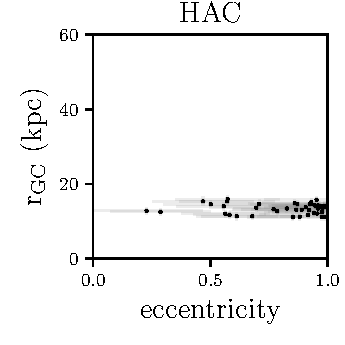
\includegraphics[scale=0.473]{HAC_orbits_ecc_r.pdf} \\
	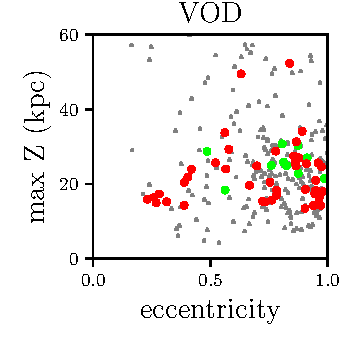
\includegraphics[scale=0.473]{VOD_orbits_ecc_z.pdf}
    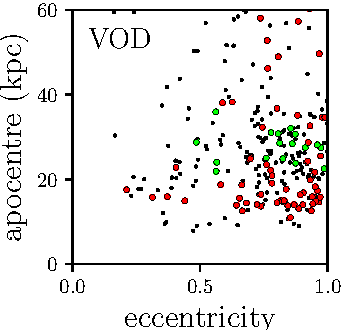
\includegraphics[scale=0.473]{VOD_orbits_apo_ecc.pdf} 
  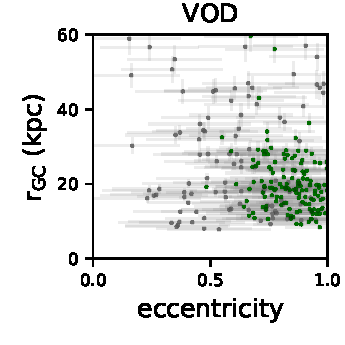
\includegraphics[scale=0.473]{VOD_orbits_ecc_r.pdf} \\
              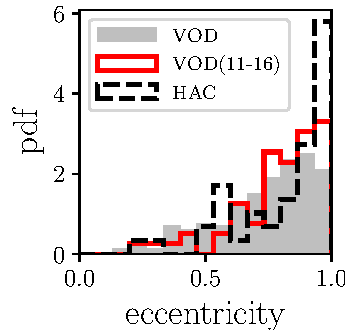
\includegraphics[scale=0.473]{eccentricities.pdf} 
    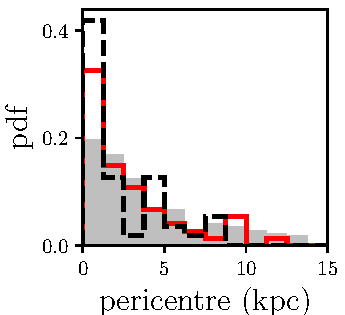
\includegraphics[scale=0.473]{pericentres.pdf} 
                          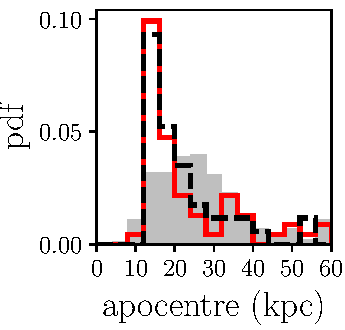
\includegraphics[scale=0.473]{apocentres.pdf} 
\vspace{-0.4cm}
  \caption{ Orbital properties of the stars in the HAC and VOD fields. `group 2' has similar orbital properties to the HAC, however it does not display a sausage velocity distribution (see middle row figure 2) - they are concentrated at $vr =  135 $km/s as calculated by Vivas et al. 2016. }
    \label{fig:orbits}
    
    \end{figure}
   %
For orbit integration we use the $\mathrm{galpy}$ package \citet{Bovy2015} in the recommended  $\mathrm{MWPotential2014}$ model for the Galactic potential which is composed of a Miyamoto-Nagai disc, a bulge with a power-law density profile that is exponentially cut-off, and a dark matter halo described by a NFW potential. The parameters are given in \citet{Bovy2015}, table 1. The resulting orbital parameters of the HAC and VOD are given in Fig \ref{fig:orbits}. To compute the errors (not shown for VOD to simply the figure) we integrated 500 orbits for each star where the orbits were initialised on parameters resampled from data, as in the previous section. The pdfs of the eccentricities, apocentres and pericentres are also shown.
If the HAC orbits are clearly highly eccentric, we find that the majority of stars in VOD are also on quite eccentric orbits: in particular, the stars with $11<\mathrm{r_{GC}}$/kpc$<16$ (in red), follow closely the HAC orbital properties.
%
\section{Are the VOD and the HAC related?}
In this section we discuss the possible connection between the two clouds. 
We use the 6-D phase space measurements as initial conditions for backward orbit integration. We integrate the orbits for 8 Gyrs %here need to discuss why.
and show them in Fig. \ref{fig:backorbits}.


\begin{figure*}
	     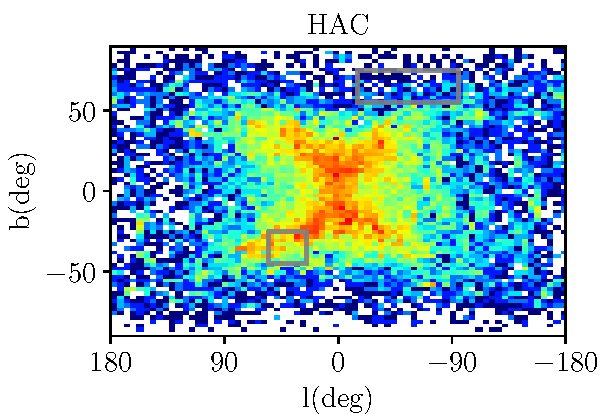
\includegraphics[scale=0.52]{HAC_orbits_8Gyrs_lb_defaultmass.pdf}
	     	     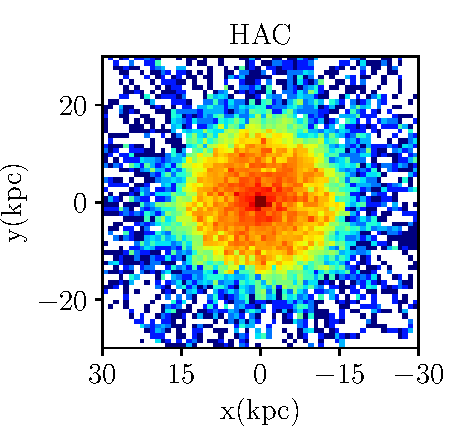
\includegraphics[scale=0.52]{HAC_orbits_8Gyrs_xy_defaultmass.pdf}
	     	     	     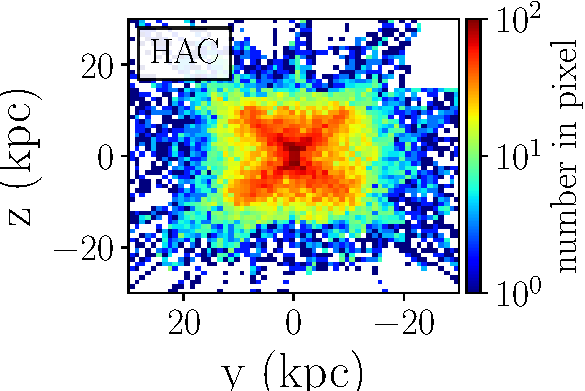
\includegraphics[scale=0.52]{HAC_orbits_8Gyrs_yz_defaultmass.pdf}
	     	     	     	     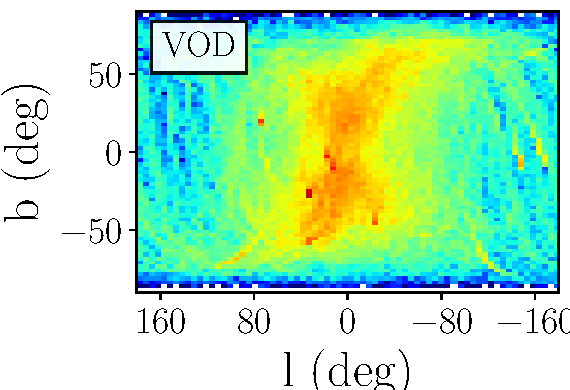
\includegraphics[scale=0.52]{VOD_orbits_8Gyrs_lb_defaultmass.pdf}
	     	     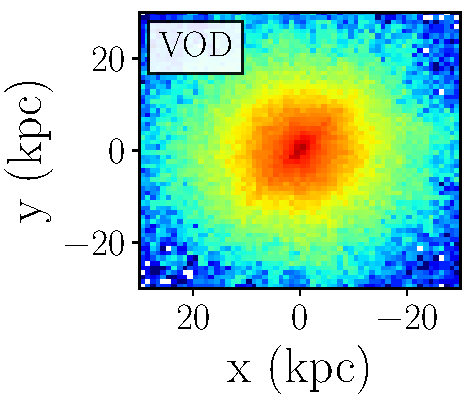
\includegraphics[scale=0.52]{VOD_orbits_8Gyrs_xy_defaultmass.pdf}
	     	     	     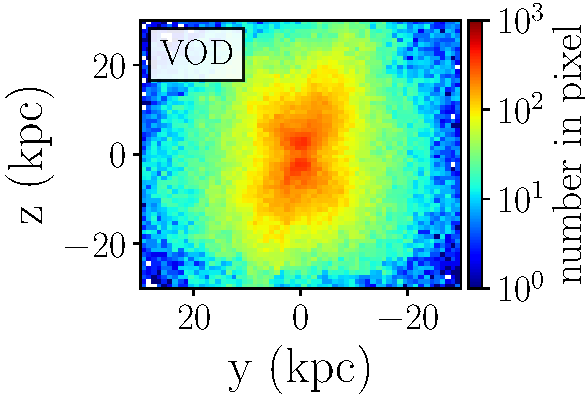
\includegraphics[scale=0.52]{VOD_orbits_8Gyrs_yz_defaultmass.pdf}
	     	     	     	     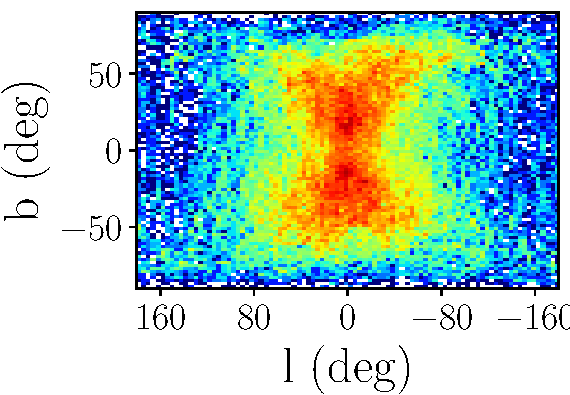
\includegraphics[scale=0.52]{VOD_orbits_8Gyrs_lb_sausage.pdf}
	     	     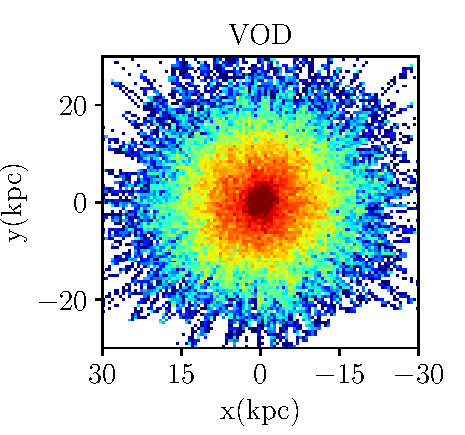
\includegraphics[scale=0.52]{VOD_orbits_8Gyrs_xy_sausage.pdf}
	     	     	     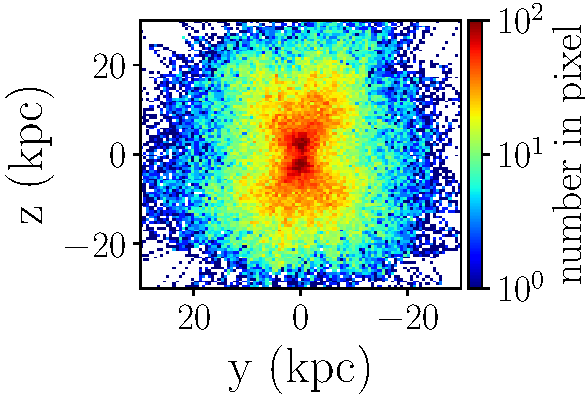
\includegraphics[scale=0.52]{VOD_orbits_8Gyrs_yz_sausage.pdf}
   \caption{The backward orbit integration for HAC (top panels) and VOD (bottom panels) for 8 Gyrs look back time. We use $M_{vir} = 0.8 \times 10^{12} M_{\odot}$, the default galpy value . log(N) shown, notice the change in colour scale between top and bottom rows. The present day loci of  HAC and VOD are marked with gray rectangles. The initial conditions of 44 stars with heliocentric distances between 15 and 18 kpc were used for the HAC backward orbit integration and of 299 stars with heliocentric distances between 4 and 75 kpc for the VOD orbit integration.}
    \label{fig:backorbits}
\end{figure*}
\begin{figure}
	% To include a figure from a file named example.*
	% Allowable file formats are eps or ps if compiling using latex
	% or pdf, png, jpg if compiling using pdflatex
	       	       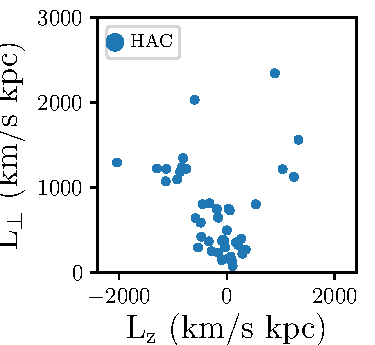
\includegraphics[scale=0.52]{HAC_Lz_Lp.pdf}
	       	       	       	       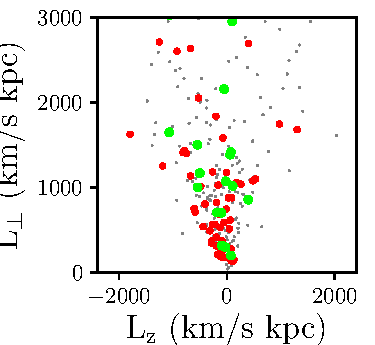
\includegraphics[scale=0.52]{VOD_Lz_Lp.pdf}
   \caption{EXTRA: angular momentum - I can combine these two and also add another panel with energy vs total L when I figure out the energy.}
    \label{fig:l}
\end{figure}
\section{Conclusions}

Using a sample of $\sim$500 RR Lyrae with full 6-D phase space
information, we have studied the orbital properties of the
Hercules-Aquila and Virgo Clouds. Both Clouds appear dominated by
stars on highly eccentric orbits. Assuming that the kinematics of each
structure is well described by a single Gaussian, the orbital
anisotropy of the HAC is $\beta=0.91$ and for the VOD,
$\beta=0.74$. Note, however that the original criteria applied to the
RR Lyrae stars to select targets for spectroscopic follow-up differ
drastically between the HAC and the VOD datasets. The HAC sample
covers a very limited region in the of $l,b, D$ space, while the VOD
dataset spans a wide range of longitudes, latitudes and heliocentric
distances. It is therefore likely that the VOD dataset contains a
mixture of several halo sub-structures \citep[see][for a detailed
  discussion]{Vivas2016}. For the entirety of the analysis described
here, we made sure to cull the probable Sgr stream
members. Additionally, we explore how the VOD's make-up changes with
Galactic height and demonstrate that for $|z|<20$ kpc, the VOD orbital
anisotropy is $\beta\sim 0.84$, while above this threshold, it quickly
changes to $\beta\sim0$. We conclude therefore, that an assumption of
a single Gaussian for the entire VOD sample is not
appropriate. Modeling the kinematics of the VOD stars with a mixture
of 2 multi-variate Gaussians, we show that two thirds of the VOD
sample are the stars with $\beta=0.96$, while the remainder has
$\beta=0.44$, in good agreement with the local measurement presented
in \citet{Belokurov2018}.

As revealed by Gaia, the two structures are composed of stars on
nearly radial orbits, with peaks in the eccentricity distribution at
0.9 (0.8) for the HAC (VOD). The distributions of the peri-centric and
apo-centric distances also match: the stars in the Clouds turn around
at $1-3$ and $15-30$ kpc. Not only the HAC and the VOD look alike
kinematically, their orbital composition is in perfect agreement with
the stellar halo properties as analysed locally by
\citet{Belokurov2018} and globally (out to 40 kpc) by
\citet{Deason2018pileup}. As these authors demonstrate, the inner halo
is dominated by metal-rich debris from an old and massive accretion
event. In particular, \citet{Belokurov2018} use Cosmological
simulations of Milky Way halo formation, to bracket the time of the
merger - between 8 and 11 Gyr ago - and its mass, which they show to
be in excess of $10^{10} M_{\odot}$. The tell-tale sign of this
dramatic head-on collision is the particular shape of the
corresponding stellar velocity ellipsoid, which is stretched so much
in the radial direction compared to the tangential ones, that it
resembles a sausage. An alternative view of this merger can be found
in \citet{actionhalo}, where the local stellar halo is mapped out in
the action space. Here, the metal-rich stars are shown have extended
radial action distribution in addition to a prominent spray of
material on retrograde orbits. The high mass of the progenitor is
evidenced not only by the metallicity distribution of its likely
member or the numerical simulations of halo formation, but also by a
sizeable number of Globular Clusters that could be attributed to the
same event \citep[see][]{sausagegc}.

\citet{Jo2012} attempted to connect various clouds together.

\section*{Acknowledgements}

The research leading to these results has received funding from the
European Research Council under the European Union's Seventh Framework
Programme (FP/2007-2013) / ERC Grant Agreement n. 308024.


%%%%%%%%%%%%%%%%%%%%%%%%%%%%%%%%%%%%%%%%%%%%%%%%%%

%%%%%%%%%%%%%%%%%%%% REFERENCES %%%%%%%%%%%%%%%%%%

% The best way to enter references is to use BibTeX:
%citations used: 
\bibliographystyle{mn2e}
\bibliography{bibl}  %the same name as the tex file
%%%%%%%%%%%%%%%%%%%%%%%%%%%%%%%%%%%%%%%%%%%%%%%%%%
% Don't change these lines
\bsp	% typesetting comment
\label{lastpage}
\end{document}
% End of mnras_template.tex
